\section{HAMMER System Architecture}
\label{sec:architecture}

\hammer{} is an implemented application: a Python service built on FastAPI with an SQLite relational store, a persistent vector index, and a React front end. This section describes the components that exist in the code base and says which of them take part in the author-resolution experiment of Section~\ref{sec:design}. Many do not, and the description of a component is not a claim that it was evaluated. Fig.~\ref{fig:architecture} gives the overview and Table~\ref{tab:components} lists responsibilities.

The architecture has two levels that share no scores. The \emph{work level} decides whether provider records describe the same publication. The \emph{person level} proposes provider author profiles for a name and decides whether one of them may be assigned. Publication-matching outputs, such as a merged record's confidence field, are not inputs to the author decision, and author scores are not inputs to deduplication.

\begin{figure*}[t]
\centering
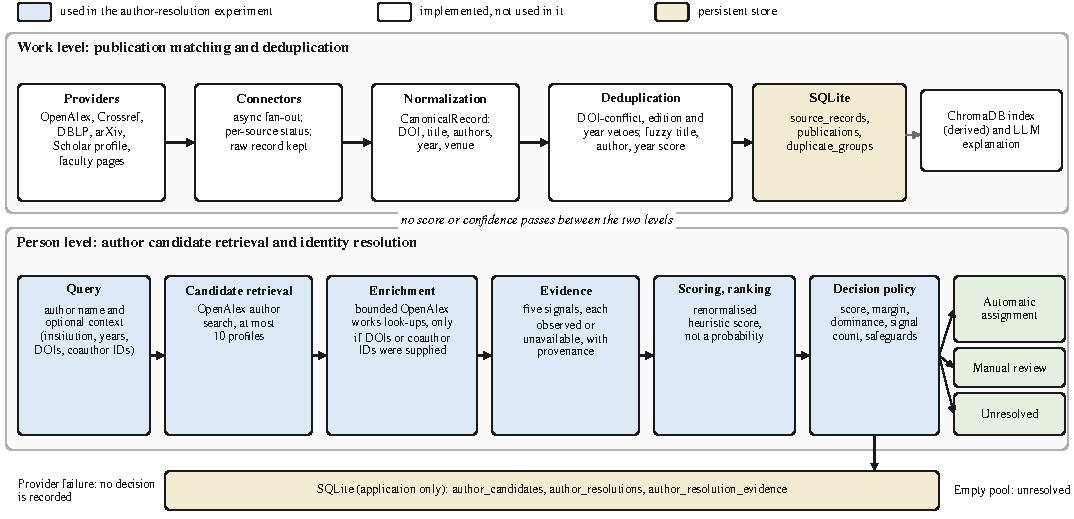
\includegraphics[width=\textwidth]{figures/architecture.pdf}
\caption{\hammer{} architecture. The work level (top) and the person level (bottom) are separate pipelines. Blue boxes take part in the author-resolution experiment; white boxes are implemented but are not used in it. The offline replay reads captured provider responses and neither reads nor writes the databases. Regenerate with \texttt{figures/make\_figures.py}.}
\label{fig:architecture}
\end{figure*}

\begin{table*}[t]
\caption{Components, responsibilities and role in the author-resolution experiment.}
\label{tab:components}
\centering
\footnotesize
\renewcommand{\arraystretch}{1.12}
\begin{tabular}{@{}p{0.17\textwidth}p{0.53\textwidth}p{0.22\textwidth}@{}}
\toprule
\textbf{Component} & \textbf{Responsibility} & \textbf{In the experiment?} \\
\midrule
Connectors & Fetch publication records from OpenAlex, Crossref, DBLP and arXiv, from cached Google Scholar profile pages for manually mapped authors, and from a configured faculty-page scraper; return records plus a per-source status & No \\
Normalization & Map each raw record to a canonical record (DOI, title, authors, year, venue, citations, raw JSON) & No \\
Deduplication & Decide whether two records are the same work; merge by source priority & No \\
Relational store & Keep raw source records, merged publications with per-field source attribution, duplicate groups, similarity logs, and author candidates, resolutions and per-signal evidence & No (replay uses no database) \\
Candidate retrieval & Query the OpenAlex authors endpoint and parse profiles into candidates & Yes \\
Enrichment & Bounded OpenAlex works look-ups that supply publication and coauthor evidence; coauthor evidence is supported in general but cannot be obtained on LAGOS-AND & Yes (publication evidence in C1x only; no coauthor evidence) \\
Evidence, scoring & Extract five signals per candidate and combine them into a heuristic score; on LAGOS-AND at most four can be observed, because coauthor identifiers are absent & Yes (at most four signals) \\
Decision policy & Apply score, margin, dominance, signal-count and safeguard rules; return one of three outcomes & Yes \\
Manual review & API and interface for a reviewer to select a candidate or mark the query unresolved & No (implemented; not exercised by the offline replay) \\
Vector index, LLM explanation & Rebuildable ChromaDB projection of canonical publications; optional Gemini explanation with citation containment & No; not shown to affect decisions \\
Capture and replay & Record each OpenAlex response with a hash; replay the resolver offline from the records & Yes \\
\bottomrule
\end{tabular}
\end{table*}

\subsection{Scholarly Metadata Acquisition}
Each connector implements one interface that returns a list of records and a status dictionary, and records a failure in the status instead of raising it. Per-source switches select the active connectors, and a configurable timeout bounds each call (ten seconds by default). A fixed source-priority order (Crossref, OpenAlex, DBLP, arXiv, Scholar, faculty page) decides which source supplies a field when records are merged. The raw response is stored with each source record.

Acquisition is not identity verification. A publication record carries author name strings, and the connector layer does not decide whether any name refers to a particular person. The author-resolution experiment uses only the OpenAlex authors and works endpoints (Section~\ref{sec:candidates}). The other connectors, the Scholar cache and the faculty scraper take no part in it.

\subsection{Normalization and Canonical Publication Records}
Normalization converts each provider record into one canonical form before comparison. HTML tags are stripped from titles and abstracts, DOIs are lower-cased with resolver prefixes removed, a four-digit year is extracted, author lists are parsed into name strings, and the citation count is coerced to an integer. A deterministic canonical identifier is derived from the DOI when one exists and otherwise from a hash of the source identifier and the normalized title.

The relational store keeps three views of a publication: the raw source record exactly as received, the merged canonical publication with the source that supplied each field (DOI, abstract, venue, citations) and the list of contributing sources, and a duplicate-group table that maps a merged publication to its source records. Source identifiers and raw JSON therefore survive merging.

\subsection{Publication Matching and Deduplication}
Deduplication answers a work-level question: do two records describe the same publication? It compares records pairwise after a cheap blocking step. Deterministic checks can veto or force a merge: conflicting valid DOIs forbid a merge, an identical DOI forces one, explicit conflicting edition markers (for example first and second edition) forbid one, and a year gap of four or more without a matching DOI forbids one. Remaining pairs receive a weighted similarity of title, author keys and year, which is compared with a threshold that depends on the pair of sources, and a title-similarity floor stops distinct works that share keywords from merging. Pairs whose score exceeds a logging threshold are written to an audit table with the merge decision. Groups are formed by union-find.

The output is a merged publication with a confidence field that is set by the number of contributing records, not by an estimate of correctness. It describes document equivalence only. It is not an identity confidence and is not used by the author resolver. Deduplication is not the subject of the research questions studied here, and no deduplication result is reported.

\subsection{Author Candidate Retrieval}
\label{sec:candidates}
Candidate retrieval produces hypotheses and nothing more. The candidate service queries the OpenAlex authors endpoint for a name and parses each returned object into a candidate profile: the provider's author identifier, display name and aliases, affiliations (institution name, OpenAlex institution identifier and ROR identifier where present), works count, citation count, the first and last year in the profile's yearly counts, and the raw payload. Malformed items, and items without an identifier or a non-blank display name, are dropped, and duplicate identifiers are removed in first-seen order. A returned identifier identifies a provider profile. It does not establish that the profile is the person the user meant, and it does not establish identity in any other source.

Retrieval has three distinguishable outcomes: a pool of candidates, a successful empty response, and a failure (timeout, request error, rate limit, HTTP error, malformed body, empty query, or an input that looks like an institution and is refused). A failure is never reported as an empty pool. The pool holds at most ten profiles from a single page.

Retrieval, ranking and assignment are separate steps. The order in which the provider returns candidates is the order used for the retrieval metrics. Ranking happens only after evidence extraction and uses the heuristic score of Section~\ref{sec:signals}. Assignment is a further step governed by the decision policy. Separately, the publication-search path contains an older candidate picker with its own score and automatic-selection rule; it is not the resolver described here and is not evaluated.

\subsection{Evidence Enrichment and Decision Workflow}
Evidence extraction, scoring and the decision policy are pure functions: they read a candidate and the query context and never touch the network, the database or the vector index. The only component that contacts OpenAlex for works-derived evidence is the enrichment service, and it does so only when the query supplies the input that makes a retrieval useful. If the query lists publication identifiers (DOIs or OpenAlex work identifiers, at most fifty), one look-up resolves their authorships. If it lists coauthor OpenAlex author identifiers, a bounded sample of each candidate's works (at most two pages of one hundred, with an explicit sort order) supplies that candidate's coauthors. An enrichment failure never fails the pool: it is recorded against the affected signal as unavailable.

The workflow therefore runs: candidate retrieval, optional enrichment, evidence extraction, scoring and ranking, and the decision policy of Section~\ref{sec:policy}, which yields \emph{automatic assignment}, \emph{manual review}, or \emph{unresolved}. In the application, a reviewer may then select one candidate or mark the query unresolved. That reviewer decision is stored as a separate status next to the algorithmic assessment, and each response states whether the decision came from the algorithm or a reviewer. An automatic assignment creates an internal author record linked to the OpenAlex profile with a note that the link is not cross-source proof, and the record is labelled an engineering heuristic and not a confidence.

\subsection{Provenance and Traceability}
We describe only what the code stores. Each source record keeps its raw provider response. A merged publication records which source supplied each of its fields and which sources contributed. Each author candidate keeps the raw provider payload and any retrieved enrichment, with retrieval time. For each candidate and signal, the evidence table stores the availability, the signal status, the normalized score, the raw comparison values, an explanation string, the provenance of the query-side and candidate-side inputs, the effective renormalized weight and the weighted contribution. Each resolution stores the top and second score, the margin, the dominance ratio, the decision reason, and the versions of the resolver, scoring and threshold configurations.

\emph{Implementation limitation.} The schema defines a per-source authorship table intended for authorship provenance, but we found no application code that populates it. Authorship-level provenance is therefore not available from the stored data, and we make no claim that it is. For the experiment, traceability is provided at file level by the capture toolkit (Section~\ref{sec:design}): each provider response is saved with a SHA-256 hash before the next request, and the replay verifies every hash before use.

\subsection{Scope of the Experiment}
Only the person-level components marked as used in Fig.~\ref{fig:architecture} take part in the experiment, and not all five evidence signals do: coauthor evidence cannot be observed on this benchmark (Section~\ref{sec:signals}). The manual-review API and interface are implemented but are not part of the automated offline replay; the experiment scores the algorithmic outcome only and does not evaluate reviewer behaviour. The replay reads captured OpenAlex responses and does not use the relational store, the vector index or the language model. The application's candidate endpoint also returns topical retrieval hits and a model-generated explanation next to the candidates, and the code states that they do not alter the deterministic decision. We have not tested whether they help or hurt identity resolution, and no such claim is made.
